%Last updated: "Mon Jan 05 17:13:09 2004"
%modified: 2020/01/13
\documentclass[12pt,a4j,dvipdfmx,uplatex,jis2004]{jsk-thesis}

% 数式・科学表記
\usepackage{amsmath,amssymb,bm,mleftright,diffcoeff}
\usepackage{siunitx}

\usepackage{cite}
\usepackage{eclbkbox}
\usepackage{cases}
\usepackage{graphicx}
\usepackage[dvipsnames,svgnames,x11names,table,xcdraw]{xcolor}
\graphicspath{{figure/}}% includegraphicsとかのpath
\usepackage{okumacro}
\usepackage{pxrubrica}
\usepackage{url} %\url{http://hoge.ac.jp/~hoge/}
%\usepackage{html} %latex2htmlで利用
\definecolor{googleblue}{HTML}{1111cc}
\iftrue
\usepackage[dvipdfmx,%
pdflang={jp},%
bookmarks=true,%
bookmarksnumbered=true,%
bookmarkstype=toc,%
colorlinks=true,%
linkcolor=black,%
citecolor=black,%
urlcolor=googleblue,%
pdftitle={},%PDFタイトル
pdfauthor={},%PDF著者
pdfkeywords={}%PDFキーワード
]{hyperref}
\usepackage{pxjahyper}
\fi
% 相互参照
\usepackage[noabbrev]{cleveref}
% \let\nref\ref
% \let\ref\cref
% \crefname{chapter}{章}{章}
\crefformat{chapter}{#2第#1章#3}
% \crefrangeformat{chapter}{#3第#1#4--#5#2章#6}
\crefformat{section}{#2#1{}節#3}
\crefformat{subsection}{#2#1{}項#3}
\crefformat{subsubsection}{#2#1{}節#3}
\crefname{figure}{図}{図}
\crefname{table}{表}{表}
\crefname{equation}{式}{式}
\crefname{section}{}{}
\crefname{appendix}{}{}
\def\crefrangeconjunction{--}
\def\crefpairconjunction{,}
\def\crefmiddleconjunction{,}
\def\creflastconjunction{,}
\def\crefpairgroupconjunction{,}
\def\crefmiddlegroupconjunction{,}
\def\creflastgroupconjunction{,}
\usepackage{udline}

\def\topfraction{1.0}
\def\dbltopfraction{1.0}
\def\bottomfraction{1.0}
\def\dblbottomfraction{1.0}
\def\textfraction{0.0}
\def\dbltextfraction{0.0}
\def\floatpagefraction{1.0}
\def\dblfloatpagefraction{1.0}

\usepackage{pdfpages}
\usepackage{tikz,scsnowman}

% 表処理
\usepackage{booktabs}
\usepackage{multirow}

% キャプション
\usepackage{subcaption}
\captionsetup{labelsep=quad}
% \def\thesection{第\arabic{section}章}

% フォント
\usepackage[ScaleRM=1.04]{libertinus-type1}
\usepackage{libertinust1math}
\usepackage[scaled=0.93]{helvet}
\usepackage[scaled=0.91]{beramono}
\usepackage[T1]{fontenc}
% \usepackage{lmodern}
\makeatletter
\def\bfseries@rm{bx}
\makeatother

% 日本語フォント
\usepackage[expert,uplatex,bold]{otf}
% フォントを変えたいなら pxchfon パッケージを使うとよい
% 参考: https://qiita.com/zr_tex8r/items/15ec2848371ec19d45ed
\usepackage[ipaex]{pxchfon}
% \setlightminchofont{SourceHanSerifJP-Light.otf}
% \setmediumminchofont{SourceHanSerifJP-Regular.otf}
% \setboldminchofont{SourceHanSerifJP-Bold.otf}
% \setmediumgothicfont{SourceHanSansJP-Regular.otf}
% \setboldgothicfont{SourceHanSansJP-Bold.otf}
% \setxboldgothicfont{SourceHanSansJP-Heavy.otf}
% \setmarugothicfont{GenJyuuGothic-Monospace-Regular.ttf}
% \usepackage{plext}

% 脚注
\let\oldthefootnote\thefootnote
\def\thefootnote{{\color{darkgray}\oldthefootnote}}
\let\oldthempfootnote\thempfootnote
\def\thempfootnote{{\color{darkgray}$\dagger$\arabic{mpfootnote}}}
\renewcommand{\footnoterule}{\noindent\tikz\draw[dotted,darkgray] (0,0)--(5,0);\vspace{5pt}}

% jsclasses 用 mpfootnotemark
\makeatletter
\def\mpfootnotemark{%
\@ifnextchar[\@xmpfootnotemark
{\stepcounter{footnote}%
\protected@xdef\@thefnmark{\thempfn}%
\@footnotemark}}
\def\@xmpfootnotemark[#1]{%
\begingroup
\c@mpfootnote #1\relax
\unrestored@protected@xdef\@thefnmark{\thempfn}%
\endgroup
\@footnotemark}
\let\mpfootnotemarks@ve=\mpfootnotemark
\def\mpfootnotemark{\inhibitglue\mpfootnotemarks@ve}
\makeatother

% 数式略記
\DeclareMathOperator*{\argmax}{arg~max}
\DeclareMathOperator*{\argmin}{arg~min}
\DeclareMathOperator{\tr}{tr}
\newcommand{\paren}[1]{\mleft(#1\mright)}
\newcommand{\sbra}[1]{\mleft\lbrack#1\mright\rbrack}
\newcommand{\cbra}[1]{\mleft\lbrace#1\mright\rbrace}
\newcommand{\abs}[1]{\mleft|#1\mright|}
\newcommand{\norm}[1]{\mleft\|#1\mright\|}
\newcommand{\relmiddle}[1]{\mathrel{}\middle#1\mathrel{}}
\newcommand{\agivenb}[2]{#1\relmiddle|#2}
\newcommand{\agivenbp}[2]{\paren{\agivenb{#1}{#2}}}

\usepackage{bxtexlogo,strike}

\newcommand{\enhance}[1]{{\gtfamily\sffamily#1}}

% !TEX root = ../main.tex
%\setlength{\textwidth}{15cm}
%\setlength{\textheight}{33\baselineskip}
%\setlength{\textwidth}{15cm}

\newcommand{\IIC}{I\raisebox{0.8ex}{\small 2}C}
%\newcommand{\figref}[1]{{\bf Figure~\ref{fig:#1}}~}
%\newcommand{\tabref}[1]{{\bf Table~\ref{#1}}~}
%\newcommand{\equref}[1]{{\bf Equation~\ref{#1}}~}
\newcommand{\figref}[1]{{図\ref{#1}}~}
\newcommand{\tabref}[1]{{表~\ref{#1}}~}
\newcommand{\equref}[1]{{式~\ref{#1}}~}
\newcommand{\chapref}[1]{第\ref{#1}章}
\newcommand{\secref}[1]{\ref{#1}節}
\newcommand{\sgn}{\mbox{sgn}}

%\newcommand{\eqref}[1]{式(\ref{eq:#1}) }
\newcommand{\bmath}[1]{\mbox{\boldmath $#1$}}

%%\pagestyle{fancyplain}
%
%\setlength{\baselineskip}{8mm}
%\setlength{\evensidemargin}{-3mm}
%\setlength{\oddsidemargin}{10mm}
%\setlength{\topmargin}{5mm}
%\setlength{\textheight}{33\baselineskip}
%\setlength{\textwidth}{15cm}
%
%\def\chapapp#1{第#1章 :}
%\renewcommand{\chaptermark}[1]{\markboth%
%{--- \chapapp{\thechapter}#1 ---}
%{--- \chapapp{\thechapter}#1 ---}}
%\renewcommand{\chaptermark}[1]{}
%\renewcommand{\sectionmark}[1]{}
%%\setlength{\headrulewidth}{1.0pt}
%\setlength{\headsep}{15mm}
%%\setlength{\footrulewidth}{0pt}
%%\setlength{\plainheadrulewidth}{0pt}
%%\setlength{\plainfootrulewidth}{0pt}
%%\addtolength{\headwidth}{\marginparsep}
%%\setlength{\headwidth}{\textwidth}
%%\lhead[\fancyplain{}{\bf\thepage}]{\fancyplain{}{\bf\leftmark}}
%%\chead{}
%%\rhead[\fancyplain{}{\bf\rightmark}]{\fancyplain{}{\bf\thepage}}
%%\lfoot{}
%%\cfoot{}
%%\rfoot{}
%
\newcommand{\pic}[4]{%
  \begin{figure}[htbp]%
    \begin{center}%
      \includegraphics[width=#2]{#1.#4}%
    \end{center}%
   \vspace{-5mm}
    \caption{#3}%
    \label{fig:#1}% 引用は\cite{hoge}
   \vspace{5mm}
  \end{figure}}

\newcommand{\pdf}[3]{%
  \pic{#1}{#2}{#3}{pdf}
}

\newcommand{\jpg}[3]{%
  \pic{#1}{#2}{#3}{jpg}
}

% \newcommand{\fig}[3]{%
%   \pic{#1}{#2}{#3}{eps}
% }

\newcommand{\png}[3]{%
  \pic{#1}{#2}{#3}{png}
}

% \newcommand{\figs}[5]{%
%   \begin{figure}[htbp]%
%     \leavevmode
%     \begin{center}%
%       \includegraphics[width=#2]{figure/#1.eps}%
%       \includegraphics[width=#4]{figure/#3.eps}%
%     \end{center}%
%     \vspace{-5mm}
%     \caption{#5}%
%     \label{fig:#1}% 本文で引用するときは\cite{fig:hoge}なので注意
%     \vspace{5mm}
%   \end{figure}}

% \newcommand{\twofigs}[6]{%
%   \begin{figure}[htbp]%
%     \begin{minipage}{0.5\hsize}%
%       \begin{center}%
%         \includegraphics[width=#2]{figure/#1.eps}%
%       \end{center}%
%       \caption{#3}%
%       \label{fig:#1}% 本文で引用するときは\cite{fig:hoge}なので注意
%     \end{minipage}%
%     \begin{minipage}{0.5\hsize}
%       \begin{center}%
%         \includegraphics[width=#5]{figure/#4.eps}
%       \end{center}%
%       \caption{#6}%
%       \label{fig:#4}% 本文で引用するときは\cite{fig:hoge}なので注意
%     \end{minipage}%
%   \end{figure}}

\newcommand{\twofigure}[3]{%
\begin{figure}\centering\begin{minipage}[b]{.5\linewidth}\centering #1\end{minipage}%
\begin{minipage}[b]{.5\linewidth}\centering #2\end{minipage}#3\end{figure}}
\newcommand{\twofigurec}[3]{%
\begin{figure*}\centering\begin{minipage}[b]{.5\linewidth}\centering #1\end{minipage}%
\begin{minipage}[b]{.5\linewidth}\centering #2\end{minipage}#3\end{figure*}}
\newcommand{\twofiguret}[3]{%
\begin{figure}\centering\begin{minipage}[b]{\linewidth}\centering #1\end{minipage}\\%
\begin{minipage}[b]{\linewidth}\centering #2\end{minipage}#3\end{figure}}

\RequirePackage{color}\definecolor{RED}{rgb}{1,0,0}\definecolor{BLUE}{rgb}{0,0,1}
%\providecommand{\DIFadd}[1]{{\protect\color{blue} \protect\ul{#1}}}
%\providecommand{\DIFadd}[1]{{\protect\color{blue} \fontsize{10.5pt}{0pt}#1}}
%\providecommand{\DIFdel}[1]{{\protect\color{red} \footnotesize \protect\Sl{#1}}}
%\providecommand{\DIFdel}[1]{{\protect\color{red} \footnotesize #1}}
\providecommand{\DIFaddbegin}{}
\providecommand{\DIFaddend}{}
\providecommand{\DIFdelbegin}{}
\providecommand{\DIFdelend}{}
\providecommand{\DIFaddFL}[1]{\DIFadd{#1}}
\providecommand{\DIFdelFL}[1]{\DIFdel{#1}}
\providecommand{\DIFaddbeginFL}{}
\providecommand{\DIFaddendFL}{}
\providecommand{\DIFdelbeginFL}{}
\providecommand{\DIFdelendFL}{}


\date{平成27年2月2日 提出}
\author{指導教員 hogehoge~教授\\~\\~\\~\\東京大学大学院~情報理工学系研究科~知能機械情報学専攻\\00-000000~hogehoge}
\title{タイトル\\
\scsnowman[scale=2,body,hat=red,muffler=blue]\scsnowman[scale=2,hat,snow,arms,buttons,note]\scsnowman[scale=3,muffler=red,arms,broom=brown]\scsnowman[scale=2,mouthshape=frown,hat=green]\ajSnowman}

\begin{document}

\setlength{\baselineskip}{20pt}

\maketitle

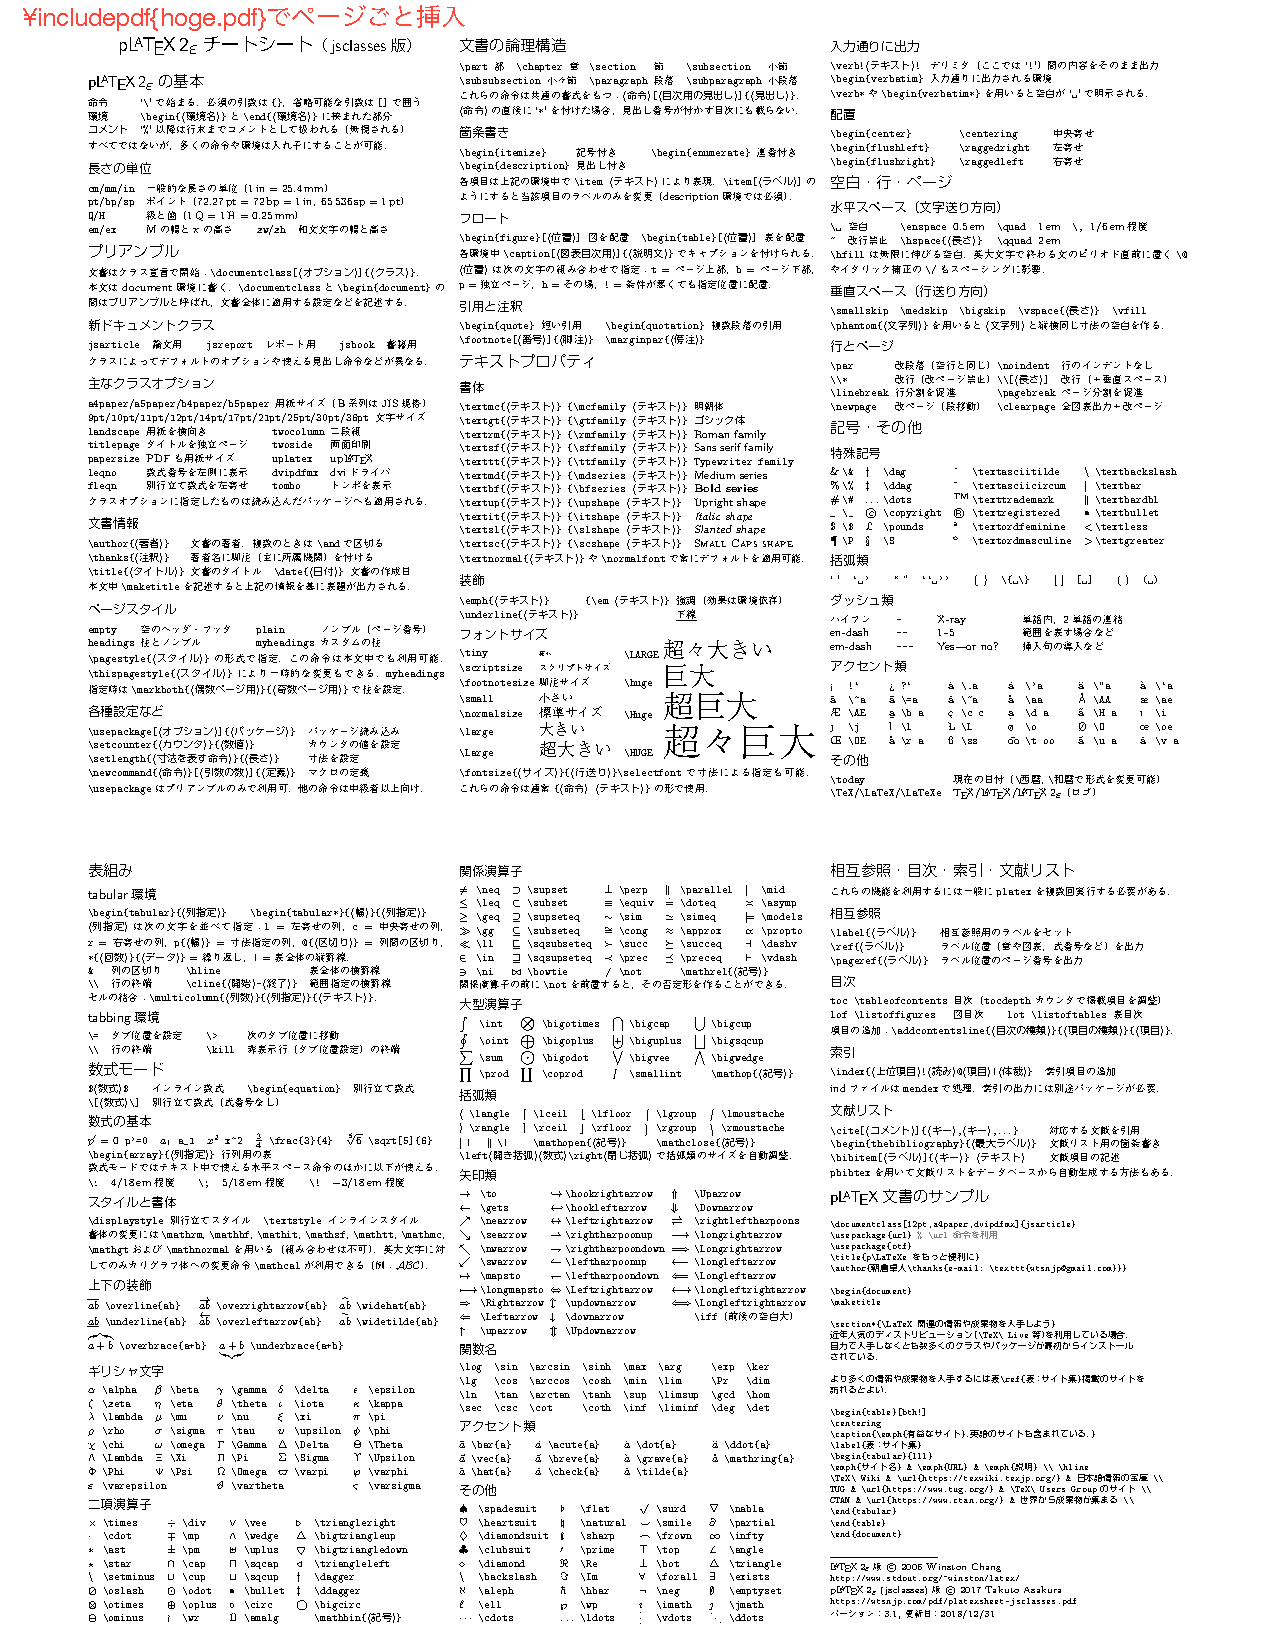
\includepdf{platexsheet-jsclasses.pdf}

\setcounter{tocdepth}{1}
\tableofcontents
% \listoffigures
% \listoftables

% !TEX root = ../main.tex
%Last updated: "Mon Jan 05 23:25:33 2004"
%\documentclass[12pt]{jsk-thesis}
%\begin{document}

\chapter{序論}
\label{chap:introduction}
\section{このテンプレートについて}
%%%%%%%%%%%%%%%%%%%%%%%%%%%%%%%%%%%%%%%%%%%%%%%%%%%%%%%%%%
お\TeX\TeX\ \ \upLaTeX\ \ \pLaTeX
\par
jskのやつと\href{https://github.com/Ishotihadus/master-thesis-format}{ishotihadusさんのやつ}を組み合わせてみた.\\
macOS Montereyのtexlive(mactex)2021で動作確認した.
\subsection{主張}
makefileやepsは使わないようにしましょう.latexmkrcを環境や好みに合わせて変更し,\texttt{latexmk -pvc}でプレビューしながらやると便利.プリアンブルがchapters/00preamble.texとmain.texに分かれてるのは申し訳ない.自分で使いたいパッケージがあればどちらかに書けばよいが,たまにusepackageの順番の前後で動作が変わるものがあるので注意.
\subsection{フォントについて}
main.texの真ん中らへんのところを好きにいじるとよい.

以下ishotihadusさんのテンプレートから引用(一部改変)\\
\hrulefill
\section{このフォーマットの使い方}

\label{sec:02-hoge}

\subsection{動作環境}

\TeX Live 2018の\upLaTeX を使っている.
こういうのはなるべく新しいものを使ったほうがいいぞ.
\upLaTeX を使うことで,種﨑敦美みたいな文字を普通に出せるようになる.

\subsection{latexmk}

latexmkrcに必要なことは書いてあるので,latexmkを走らせればpdfが作れる.はず.

\subsection{atom-latex}

Atomのlatexパッケージ\footnote{\url{https://atom.io/packages/latex}}に対応している.
各ファイルの先頭にある\verb|% !TEX|の行は,このパッケージ用のマジックコメントである.

\subsection{ファイル分割}

さすがに大きいと面倒くさそうなのでファイルを分割している.
簡単なのでinputコマンドを使っているが,subfilesなどを利用してもよい.

各ファイルの先頭の\verb|% !TEX root = ../main.tex|のマジックコメントは,書いておくとこのファイルを開いてコンパイルを走らせても勝手にmainがコンパイルされるようにするもの.

\subsection{フォント}
\label{ssec:02-hoge-font}

日本語フォントは各自設定すること.
データも提出するはずなので,フォントの埋め込みは忘れずに.
フォントが埋め込まれているかどうかはAdobeのAcrobatとかでプロパティを見るとわかる.

欧文フォントも日本語に合わせて適当に変えるとよい.
設定するときは\LaTeX Font Catalogue\footnote{\url{http://www.tug.dk/FontCatalogue/}}などを参考にするとよい.

フォントサイズは\verb|documentclass|のオプションで指定する.
指定なし(10pt)にするとPostScript換算で\SI{9.21}{pt}(\SI{9.21}{bp})になってしまって少し小さいので,10ptjを指定して\SI{10}{bp}にしている.

jsclassesでの最新版では,8pt,9pt,10pt,11pt,12pt,14pt,17pt,20pt,21pt,25pt,30pt,36pt,43pt,12Q,14Q,10ptj,10.5ptj,11ptj,12ptjが使える.
\pLaTeX での\SI{10}{pt}は\SI{13}{Q}のことで,14Qを指定すると\pLaTeX での$10 \times 14/13=\SI{10.77}{pt}$になる.
10ptj(\SI{10}{bp})は,\pLaTeX では\SI{10.85}{pt}になる.

\subsection{コマンドの使い方}
\label{ssec:02-hoge-commands}

便利なコマンドをちょこちょこ用意したので使ってほしい.

\subsubsection{数式}

argminやargmaxはコマンドを作ってあるのでそれを使うとよい.
\begin{equation}
    \hat{x} = \argmin_{x} f(x)
    \label{eq:eq1}
\end{equation}

括弧はparen,cbra,sbraコマンドを使うと\verb|\left( \right)|などと同じ処理になる.
\begin{equation}
    i\hbar\diffp*{\psi\paren{\bm{x},t}}{t} = \sbra{\frac{-\hbar^2}{2m}\nabla^2 + V\paren{\bm{x},t}}\psi\paren{\bm{x},t}
    \label{eq:eq2}
\end{equation}
同様にabs,normコマンドもある.
\begin{equation}
    \abs{\jacob{x,y}{r,\theta}} = r
    \label{eq:eq3}
\end{equation}
\begin{equation}
    \norm{A}_F = \sqrt{\sum_{i=1}^m\sum_{j=1}^n\abs{a_{ij}}^2}
    \label{eq:eq4}
\end{equation}

条件付き確率を書くためだけのagivenbとagivenbpコマンドもある.
pが付いている方は括弧もついでに書く.
\begin{equation}
    p\agivenbp{\bm{x}}{\bm{\alpha}} = \frac{\Gamma\paren{\prod^P\alpha_p}}{\prod_p^P\Gamma\paren{\alpha_p}}\prod_p^Px_p^{\alpha_p-1}
    \label{eq:eq5}
\end{equation}

偏微分はdiffcoeffパッケージを使っている.
diffcoeffでググると僕の記事が上の方に出てくるので使うとよい.

\begin{equation}
    \kappa_n = \diff[n]{K_X(t)}{t}[t=0] = \begin{cases}
        \mu+\gamma\eta & (n=1) \\
        \eta^k(n-1)!\zeta(n) & (n \geq 2)
    \end{cases}
    \label{eq:eq6}
\end{equation}

\subsubsection{文字の強調}

enhanceコマンドで文字列が\enhance{このようにゴシック体になってstrongになる}ようになっている.
名前がstrongじゃないのはなんか他のパッケージとぶつかるからだった気がする.

\subsubsection{URL}

urlパッケージをデフォルトで読み込んである。urlコマンドでURLがなんかいい感じに出力される.

\subsubsection{subfigure}

2つ画像を並べるときがときどきあるので,それ用のコマンドを用意してある.
\ref{fig:yayoiori}にその例を示す.

\twofigure{
    
\includegraphics[width=.8\linewidth]{star.png}
    \subcaption{star}
    \label{fig:iori}
}{
    
\includegraphics[width=.8\linewidth]{moon.png}
    \subcaption{moon}
    \label{fig:yayoi}
}{
    \caption{star and moon}
    \label{fig:yayoiori}
}

\subsection{参照}

あらゆる参照はcrefコマンドだけでOKなようになっている.
「図」とか「表」とか「節」とか「式」とかは空気を読んで勝手に入る.

\cref{fig:kana}にcatの画像を示す.
また,最近のフェス限の性能比較は\cref{tbl:fes}に示す.

\begin{figure}
    \centering
    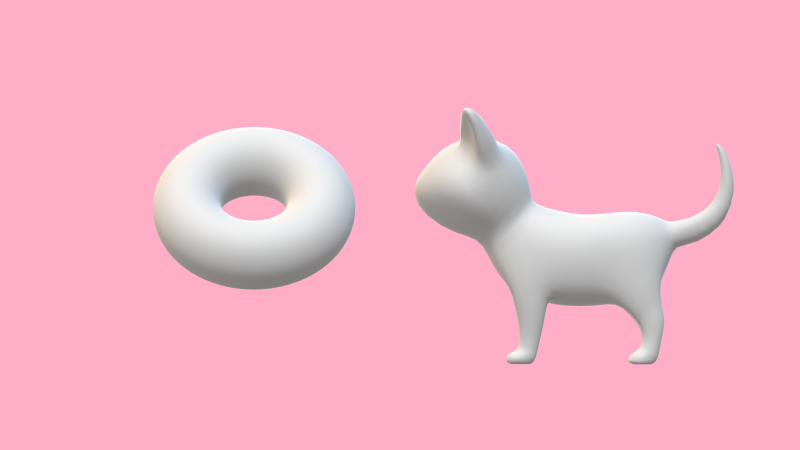
\includegraphics[width=.8\linewidth]{cat.png}
    \caption{cat}
    \label{fig:kana}
\end{figure}

\begin{table}
    \centering
    \caption[フェス限やよいおりとかなしほの性能比較]{フェス限やよいおりとかなしほの性能比較(すべて特訓後☆4時).センターに配置すると,特化値が+95\%されることに留意する.こう見ると伊織が結構弱い.}
    \begin{tabular}{cc|cccc|crcc}
        \toprule
        アイドル & タイプ & Vo & Da  & Vi & 合計 & 特技 & 間隔 & 確率 & 時間 \\ \hline\hline
        矢吹可奈 & Princess & 6433 & 3272 & 9630 & 19335 & \multirow{4}{*}{コンボナ28\%} & 7秒 & \multirow{4}{*}{40\%} & 4秒 \\\cline{1-6}\cline{8-8}\cline{10-10}
        北沢志保 & \multirow{2}{*}{Fairy} & 3262 & \textbf{9631} & 6454 & \textbf{19347} & & 13秒 & & 7秒 \\\cline{1-1}\cline{3-6}\cline{8-8}\cline{10-10}
        水瀬伊織 &  & 6452 & 9578 & 3216 & 19246 & & 11秒 & & 6秒 \\\cline{1-6}\cline{8-8}\cline{10-10}
        高槻やよい & Angel & 9601 & 6446 & 3280 & 19327 & & 10秒 & & 5秒\\
        \bottomrule
    \end{tabular}
    \label{tbl:fes}
\end{table}

章や節の参照は\cref{sec:02-hoge}とか\cref{ssec:02-hoge-font}とかになる.

refはcleverefを使っているので,\verb|\ref{eq:eq1,eq:eq2,eq:eq3}|などとカンマ区切りで使える.
使うと\cref{eq:eq1,eq:eq2,eq:eq3,eq:eq5}のように勝手にいい感じになる.
なお,章と節の参照をカンマ区切りで指定するとおかしくなっちゃうので,これは使わないほうがよい(設定するのが面倒くさかった).

\subsection{参考文献}

\strike{参考文献と発表文献を分けて書けるようになっている.普通にciteすると参考文献に載るようになっており,発表文献のファイルはデフォルトですべて出力されるようになっている.発表文献の順序はbibファイルに書かれている順序になる.}
\par 引用順に載るようになっている.

\subsection{脚注}

デフォルトの脚注のデザインがあまり好きじゃないのでいじってある.

\begin{center}
    \begin{minipage}{0.6\linewidth}
        \LaTeX{}では,minipage環境内で別の脚注を使うことができる.
        このテンプレートはそれにも対応している\footnote{こんな感じ.}.
        mpfootnotemarkコマンドをjsclasses用に作り変えたやつを定義してあるので,こんな感じに使える\mpfootnotemark[765].
        \footnotetext[765]{765個も脚注はない.}
    \end{minipage}
\end{center}
\hrulefill\\引用以上.


%%%%%%%%%%%%%%%%%%%%%%%%%%%%%%%%%%%%%%%%%%%%%%%%%%%%%%%%%%

% \parbox{6zw}{\ajMaru{1}横組\ajLig{サンチーム}\\
%   {\TeX}は\textbf{アレ}、\\
%   {\ajSnowman}は\textbf{非アレ}。}%
% \quad
% \parbox<t>{6zw}{\ajMaru{2}縦組\ajLig{サンチーム}\\
%   {\TeX}は\textbf{アレ}、\\
%   {\ajSnowman}は\textbf{非アレ}。}% https://zrbabbler.hatenablog.com/entry/20171008/1507481645 より引用



%%%%%%%%%%%%%%%%%%%%%%%%%%%%%%%%%%%%%%%%%%%%%%%%%%%%%%%%%%
 \section{研究の目的}
%%%%%%%%%%%%%%%%%%%%%%%%%%%%%%%%%%%%%%%%%%%%%%%%%%%%%%%%%%
% \verb|\cref{}|でいい感じに
\cref{fig:arm}のように〜
%%%図を入れる(基本)%%%
% \begin{figure}[htbp]
% \begin{center}
% 
\includegraphics[width=0.7\columnwidth ]{arm.png}
% \caption{image of arm}
% \label{fig:arm}
% \end{center}
% \end{figure}

%%%図を入れる(応用:preamble.texにショートカットコマンドを記述)%%%
\png{arm}{0.8\columnwidth}{Let's bring da house down.}

%%%%%%%%%%%%%%%%%%%%%%%%%%%%%%%%%%%%%%%%%%%%%%%%%%%%%%%%%%
\section{本論文の構成}
%%%%%%%%%%%%%%%%%%%%%%%%%%%%%%%%%%%%%%%%%%%%%%%%%%%%%%%%%%
本論文は全\ref{chap:conclusion}章から構成される.以下に各章の概要を述べ
る.

\textbf{\cref{chap:introduction}「序論」}では,
本研究の背景と目的,及び本論文の構成を述べた.
\cite{SINRIGAKU}
%5ページぐらいかな。

\textbf{\cref{chap:concept}「」}では,

%15ページぐらいかな。


\textbf{\cref{chap:app}「」}では,

%15ページぐらいかな。


\textbf{\cref{chap:experiment1}「」}では,

%20ページぐらいかな。


\textbf{\cref{chap:experiment2}「」}では,

%20ページぐらいかな。


\textbf{\cref{chap:conclusion}「結論」}では,本研究についての結論と今後の展望について述べる.

% !TEX root = ../main.tex
%Last: "Mon Jan 05 20:27:11 2004"
\chapter{aiueo}
\label{chap:concept}

%%%%%%%%%%%%%%%%%%%%%%%%%%%%%%%%%%%%%%%%%%%%%%%%%%%%%%%%%%
\section{nnnnn}
%%%%%%%%%%%%%%%%%%%%%%%%%%%%%%%%%%%%%%%%%%%%%%%%%%%%%%%%%%

\subsection{概要}

% !TEX root = ../main.tex
%Last updated: "Mon Jan 05 20:28:42 2004"
\chapter{ggg}
\label{chap:app}

%%%%%%%%%%%%%%%%%%%%%%%%%%%%%%%%%%%%%%%%%%%%%%%%%%%%%%%%%%
\section{zoizoi}
%%%%%%%%%%%%%%%%%%%%%%%%%%%%%%%%%%%%%%%%%%%%%%%%%%%%%%%%%%

% !TEX root = ../main.tex
%Last updated: "Mon Jan 05 20:34:39 2004"
\chapter{実験1}
\label{chap:experiment1}


%%%%%%%%%%%%%%%%%%%%%%%%%%%%%%%%%%%%%%%%%%%%%%%%%%%%%%%%%%
\section{仮説}
%%%%%%%%%%%%%%%%%%%%%%%%%%%%%%%%%%%%%%%%%%%%%%%%%%%%%%%%%%

%%%%%%%%%%%%%%%%%%%%%%%%%%%%%%%%%%%%%%%%%%%%%%%%%%%%%%%%%%
\section{実験}
%%%%%%%%%%%%%%%%%%%%%%%%%%%%%%%%%%%%%%%%%%%%%%%%%%%%%%%%%%
\subsection{概要}

\subsection{結果}
結果を示す.

\subsection{考察}
うわあ

% !TEX root = ../main.tex
%Last updated: "Mon Jan 05 20:34:39 2004"
\chapter{実験2}
\label{chap:experiment2}
%%%%%%%%%%%%%%%%%%%%%%%%%%%%%%%%%%%%%%%%%%%%%%%%%%%%%%%%%%
\section{uuuu}
%%%%%%%%%%%%%%%%%%%%%%%%%%%%%%%%%%%%%%%%%%%%%%%%%%%%%%%%%%

% !TEX root = ../main.tex
%Last updated: "Mon Jan 05 20:38:51 2004"
\chapter{結論}
\label{chap:conclusion}

%%%%%%%%%%%%%%%%%%%%%%%%%%%%%%%%%%%%%%%%
\section{結論}
%%%%%%%%%%%%%%%%%%%%%%%%%%%%%%%%%%%%%%%%

%%%%%%%%%%%%%%%%%%%%%%%%%%%%%%%%%%%%%%%%
\section{今後の展望}
%%%%%%%%%%%%%%%%%%%%%%%%%%%%%%%%%%%%%%%%

% !TEX root = ../main.tex
%Last updated: "Mon Jan 05 16:32:11 2004"
\phantomsection
\markboth{謝辞}{謝辞}
\chapter*{\vspace*{-7cm}謝辞}
\addcontentsline{toc}{chapter}{謝辞}
本論文は

\begin{flushright}
2015年 2月 2日 hogehoge
\end{flushright}


\phantomsection
\addcontentsline{toc}{chapter}{参考文献}
\pagestyle{myheadings}
\markboth{参考文献}{参考文献}
\bibliographystyle{junsrt}
\renewcommand{\bibname}{\vspace*{-7cm}参考文献}
\bibliography{reference}

\phantomsection
%\addcontentsline{toc}{chapter}{付録}
\appendix
% !TEX root = ../main.tex
\chapter{球面関節角度センサの計算式の導出}

\pagestyle{myheadings}
\markboth{付録}{付録}

\section*{球面関節角度センサの計算式の導出}
%\section*{ロール・ピッチ・ヨー角計算式}

\begin{figure}
 \begin{center}
%  \includegraphics[width=100mm]{pics/04/coordinates.eps}
  \caption{Coordinates of coil arrangement.}
  \label{fig:coordinates}
 \end{center}
\end{figure}

% \figref{fig:coordinates}に示すように,内側コイルa,bの法線ベクトルを$v_a,
% v_b$,外側コイルの法線ベクトルを$v_1, v_2$とする.球面関節のヨー,ピッチ,
% ロール角をそれぞれ$\alpha,\beta, \gamma$ とし,その回転行列を\bm{R}とす
% る.\figref{fig:coordinates}のように,$\alpha=\beta=\gamma=0$の際を初期
% 姿勢とし,$v_a = (1,0,0), v_b = (0,1,0)$とすると,$v_a = \bm{R}\cdot (1,0,0),
% v_b = \bm{R} \cdot (0,1,0)$となる.ある姿勢におけるコイル1
% とコイルAのなす角度を${\theta}_{1a}$, 以下同様の表記とする.
% ${\theta}_{1a}$の余弦$cos {\theta}_{1a}$は,$v_a$と$v_1$の内積から求めら
% れ,以下のようになる.但し,$C_{\theta},S_{\theta}, T_{\theta}$はそれぞれ $cos
% \theta, sin \theta, tan \theta$の略記とする.

% M1a[a,b,c] = -Cos[theta] Sin[b]+Cos[a] Cos[b] Sin[theta]
%M2a[a,b,c] = -Cos[theta] Sin[b]-Cos[a] Cos[b] Sin[theta]
%M1b[a,b,c] = Cos[b] Cos[theta] Sin[c]+(-Cos[c] Sin[a]+Cos[a] Sin[b]
%Sin[c]) Sin[theta]
%M2b[a,b,c] = Cos[b] Cos[theta] Sin[c]-(-Cos[c] Sin[a]+Cos[a] Sin[b]
%Sin[c]) Sin[theta]
%M1c[a,b,c] = Cos[b] Cos[c] Cos[theta]+(Cos[a] Cos[c] Sin[b]+Sin[a]
%Sin[c]) Sin[theta]
%M2c[a,b,c] = Cos[b] Cos[c] Cos[theta]-(Cos[a] Cos[c] Sin[b]+Sin[a]
%Sin[c]) Sin[theta]

% \begin{equation}\label{rpy1}
%  C_{1a} = - S_{\beta} C_{\omega} + C_{\alpha} C_{\beta} S_{\omega}
% \end{equation}

% \begin{equation}\label{rpy2}
%  C_{2a} = - S_{\beta} C_{\omega} - C_{\alpha} C_{\beta} S_{\omega}
% \end{equation}

% \begin{equation}\label{rpy3}
%  C_{1b} = C_{\beta} S_{\gamma} C_{\omega} + (-C_{\gamma} S_{\alpha} + C_{\alpha} S_{\beta} S_{\gamma}) S_{\omega}
% \end{equation}

% \begin{equation}\label{rpy4}
%  C_{2b} = C_{\beta} S_{\gamma} C_{\omega} - (-C_{\gamma} S_{\alpha} + C_{\alpha} S_{\beta} S_{\gamma}) S_{\omega}
% \end{equation}

% \equref{rpy1} + \equref{rpy2}より,

% \begin{equation}\label{rpy5}
%  C_{1a} - C_{2a} = - 2 S_{\beta} C_{\omega}
% \end{equation}

% \equref{rpy1} - \equref{rpy2}より,

% \begin{equation}\label{rpy6}
%  C_{1a} - C_{2a} = 2  C_{\alpha} C_{\beta} S_{\omega}
% \end{equation}

% \equref{rpy3} + \equref{rpy4}より,

% \begin{equation}\label{rpy7}
%  C_{1b} +C_{2b} = 2 C_{\beta} S_{\gamma} C_{\omega}
% \end{equation}

% \equref{rpy3} - \equref{rpy4}より,

% \begin{equation}\label{rpy8}
%  C_{1b}  - C_{2b} = 2(-C_{\gamma} S_{\alpha} + C_{\alpha} S_{\beta} S_{\gamma}) S_{\omega}
% \end{equation}

% \equref{rpy5}, \equref{rpy6}, \equref{rpy7}より,

% \begin{equation}\label{furoku:equ:pitch}
%  \large
%   S_{\beta}  = %
%   \left(
%    \frac{C_{1a}+C_{2a}}{2 C_{\omega}}
%  \right)
% \end{equation}

% \begin{equation}\label{furoku:equ:roll}
%  \large
%   S_{\gamma} = %
%   \left(
%    \frac{C_{1b}+C_{2b}}%
%    {2 C_{\omega} C_{\beta}}
%  \right)
% \end{equation}

% \begin{equation}\label{furoku:equ:yaw}
%  \large
%   C_{\alpha} = %
%   \left(
%    \frac{C_{1a} - C_{2b}}%
%    {2  S_{\omega} C_{\beta}}
%  \right)
% \end{equation}

% となる.ロール,ピッチ角については,球面関節が初期姿勢から90度以上まわり
% 込むことはなく,可動範囲が-60〜60[deg.]程度と考えると,\equref{furoku:equ:roll},
% \equref{furoku:equ:pitch}から計算可能である.

% また\equref{rpy8},\equref{equ:pitch},\equref{equ:roll}より,

% \begin{equation}\label{furoku:equ:yaw2}
%  \large
%   S_{\alpha} = %
%    \frac{1}{2}%
%    \left(
%     (C_{1a}-C_{2b}) T_{\beta} T_{\gamma} - \frac{C_{1b}-C_{2b}}{C_{\gamma}}%
%   \right)
% \end{equation}

% となる.よって\equref{furoku:equ:yaw},\equref{furoku:equ:yaw2}を用いて,全周にわたってヨー角
% $\alpha$も一意に求めることができる.

%\section*{オイラー角での計算式}
%
%%M1a[a,b,c] = -Cos[c] Cos[theta] Sin[b]+(Cos[a] Cos[b] Cos[c]-Sin[a]
%%Sin[c]) Sin[theta]
%%
%%M2a[a,b,c] = -Cos[c] Cos[theta] Sin[b]-(Cos[a] Cos[b] Cos[c]-Sin[a]
%%Sin[c]) Sin[theta]
%%
%%M1b[a,b,c] = Cos[theta] Sin[b] Sin[c]+(-Cos[c] Sin[a]-Cos[a] Cos[b]
%%Sin[c]) Sin[theta]
%%
%%M2b[a,b,c] = Cos[theta] Sin[b] Sin[c]-(-Cos[c] Sin[a]-Cos[a] Cos[b]
%%Sin[c]) Sin[theta]
%%
%%M1a[a,b,c]+M2a[a,b,c] = -2 Cos[c] Cos[theta] Sin[b]
%%
%%M1b[a,b,c]+M2b[a,b,c] = 2 Cos[theta] Sin[b] Sin[c]
%
%\begin{equation}
% M_{1a} = -C_{\gamma} C_{\theta} S_{\beta}+(C_{\alpha} C_{\beta}
%  C_{\gamma}-S_{\alpha} S_{\gamma}) S_{\theta}
%\end{equation}
%
%\begin{equation}
% M_{2a} = -C_{\gamma} C_{\theta} S_{\beta}-(C_{\alpha} C_{\beta}
%  C_{\gamma}-S_{\alpha} S_{\gamma}) S_{\theta}
%\end{equation}

\begin{equation}
M_{1b} = C_{\theta} S_{\beta} S_{\gamma}+(-C_{\gamma}
 S_{\alpha}-C_{\alpha} C_{\beta} S_{\gamma}) S_{\theta}
\end{equation}

\begin{equation}
 M_{2b} = C_{\theta} S_{\beta} S_{\gamma}-(-C_{\gamma}
  S_{\alpha}-C_{\alpha} C_{\beta} S_{\gamma}) S_{\theta}
\end{equation}

\chapter{実装に使用したライブラリ}

本研究での実装に用いたライブラリを紹介する.

\section{OpenGL}
% \chapref{chap:predict}で実装したインタフェースの3DCGレンダリングにあたり,
OpenGL\cite{OPENGL}というライブラリを用いた.

OpenGLは元々Silicon Graphics社が中心となって開発された,
CGのためのプログラミングインタフェースである.
現在はOpenGLとして標準化が行われている.
OpenGLは,テクスチャマッピングやZバッファ法,グローシェーディング,アルファブレンディングなど,
3DCGに関する機能が充実しており,
またWindowsやLinuxなどOSを選ばず動作する移植性の高いライブラリである.

\section{OPENAL}
% \chapref{chap:predict}で実装したインタフェースの3D音響レンダリングにあたり,
OpenAL\cite{OPENAL}というライブラリを用いた.

OpenALは元々Loki Software社が開発し,Loki Software社の倒産後しばらくしてCreative Technology社が主催者として開発を進めている.
マルチチャンネル3次元定位オーディオを効率よく表現することができるプログラミングインタフェースである.

距離による衰弱やドップラー効果などの機能が充実しており,またWindowsやLinuxなどOSを選ばず動作する移植性の高いライブラリである.
% \section{JOGL}
% \chapref{chap:action}で実装したインタフェースの3DCGレンダリングにあたり,
% JOGL\cite{JOGL}というライブラリを用いた.

% JOGLは,
% Javaでネイティブメソッドを実行するための
% JNI(Java Native Interface)と呼ばれるプログラミングインタフェースで,
% JavaでのOpenGLの利用を可能にしている.
% JOGLはOpenGLのほとんどの関数をラップしており,
% さらにテクスチャ入出力などのユーティリティー機能も提供している.
% またWindowsやLinux,MacOSXなど各OS用のネイティブライブラリが用意されており,
% 移植時にはネイティブライブラリだけ変更すればよく,
% コードに手を入れる必要はほとんどない.

% \section{Joystick Driver for Java}
% \chapref{chap:action}で実装したインタフェースの入力として
% ジョイスティックを使用するにあたり,
% Joystick Driver for Java\cite{JoystickDriver}というジョイスティックドライバを用いた.
% Joystick Driver for JavaはJOGL同様,JNIを利用している.
% Joystick Driver for Javaを使うことで,
% 2〜6軸のジョイスティックが扱える.
% またWindows,Linux用のネイティブライブラリが用意されている.


% !TEX root = ../main.tex
%Last updated: "Mon Jan 05 16:31:18 2004"
\thispagestyle{empty}
\LARGE
\vspace*{2cm}
以上
\begin{center}
\vspace{4cm}
\Large
1p 〜 \pageref{bktitle}p 完\\
\vspace{1cm}
修士論文\\
\vspace{1cm}
平成27年2月2日 提出\\
\vspace{5cm}
\LARGE
東京大学大学院~
情報理工学系研究科~
知能機械情報学専攻\\
00-000000 hogehoge
\end{center}
\label{bktitle}
\normalsize


\end{document}
